\documentclass{beamer}

\usepackage{amsmath}
\usepackage{url}
\usepackage{graphicx}
\usepackage{float}
\usepackage{amsthm}
\usepackage{amssymb}
\usepackage{enumerate}

\renewcommand{\Re}{\operatorname{Re}}
\renewcommand{\Im}{\operatorname{Im}}
\newcommand{\reals}{\mathbb{R}}

\usetheme{Madrid}
\usecolortheme{beaver}

\title{Characteristic Functions}
\author[Fu\and Yao\and Zhao]{Fu Tianwen \and Yao Chaorui \and Zhao Feng}
\institute[CUHK]{the Chinese University of Hong Kong}

\begin{document}
\begin{frame}
	\titlepage
\end{frame}
\section{Problems}
\begin{frame}{Raindrops Again and Again and ...}
	\begin{block}{Raindrops in two seconds}
		Rain falls on your head at $\lambda$ drops per second on average. What is the distribution of rain drops on your head in two seconds?\pause
	\end{block}
	Our intuition tells us that it should be $Poisson(2\lambda)$.\pause
	But why?
\end{frame}
\begin{frame}{Sum of Independent Normals}
	\begin{block}{The Normal Sum Problem}
		$X_1\sim N(\mu_1,\sigma_1^2), X_2\sim N(\mu_2,\sigma_2^2).$ $X_1,X_2$ are independent. Distribution of $Y=X_1+X_2$?\pause
	\end{block}
	Observation:
	\begin{itemize}
		\item $E[Y] = E[X_1]+E[X_2]$ 
		\item $Var[Y] = Var[X_1]+Var[X_2]$ \pause
	\end{itemize}
	But what is the distribution?
\end{frame}
\section{Characteristic Functions}
\begin{frame}{Characteristic Functions}
	To deal with the sums of random variables, \textbf{characteristic function} is a powerful weapon for us.
		\begin{definition}
			Let $X$ be a random variable and denote by $F$ the cumulative distribution function of $X$ (or $f$ the probability density function). The characteristic function $\varphi=\varphi_X$ of $X$ (or of $F$, in which case we also write $\varphi_F$) is defined by
			$$\varphi_X(t):=E[e^{itX}]=\int_{-\infty}^\infty e^{itx}dF(x)=\int_{-\infty}^\infty e^{itx}f(x)dx, t\in\reals$$
		\end{definition}
\end{frame}
\begin{frame}{Recall Complex Numbers}
	If you have forgotten everything about complex numbers, all you need to recall is the following:
	\begin{itemize}
		\item $i$ is the imaginary unit,
		\item $i^2=-1$,
		\item $e^{i\theta} = \cos\theta + i\sin\theta$. (This formula comes from Taylor Series)
	\end{itemize}
\end{frame}
\begin{frame}{Properties}
	\begin{theorem}[Uniqueness Theorem]
		Let $X$ be a real random variable with distribution function
		$F$ and characteristic function $\varphi$. Similarly, let $Y$ have distribution
		function $G$ and characteristic function $\psi$. If $\varphi(t) = \psi(t)$ for all $t\in\reals$
		then $F(x) = G(x)$ for all $x \in\reals$.
	\end{theorem}
		From this we may easily conclude the distribution of a random variable if we can prove that its characteristic function is of the same form as a known distribution.
\end{frame}
\begin{frame}{Properties}
	Even if we cannot find the distribution in the lookup table, we may also retrieve it from characteristic functions by hand: \pause
	\begin{theorem}[Inversion Formula]
		If $\int_\reals |\varphi(t)| dt < \infty$ then $X$ has bounded continuous density
		$$
		f(x) = \frac1{2\pi} \int_\reals e^{-itx}\varphi(t)dt
		$$
	\end{theorem}
\end{frame}
\begin{frame}{Properties}
\begin{theorem}
	If $X$ and $Y$ are independent random variables then the characteristic function of their sum is
	$$\varphi_{X+Y}(t) = \varphi_{X}\cdot\varphi_{Y}.$$
\end{theorem}
	This gives us a much simpler way than convolution.\\\pause
	If $X$ and $Y$ are random variables such that $\varphi_{X+Y} = \varphi_X\cdot\varphi_Y $, then in general we do not conclude $X$ and $Y$ are independent. This is called \textbf{subindependence}.
\end{frame}
\begin{frame}{Properties}
\begin{theorem}
	For any $a,b \in \reals$, $$\varphi_{aX+b}(t)=e^{ibt}\varphi_X(at).$$
\end{theorem}
\end{frame}
\section{Distributions and Their Characteristic Functions}
\begin{frame}{Distributions and Their Characteristic Functions}
	\begin{example}[Characteristic Function for Exponential]
		Find the characteristic function for $X\sim Exponential(\lambda)$.
	\end{example}\pause
	$$
	\begin{aligned}[t]
	\varphi_X(t) &:=E[e^{itX}] &\\
	&=\int_{-\infty}^\infty e^{itx}f(x)dx & \\
	&=\int_0^\infty e^{itx}\cdot \lambda e^{-\lambda x}dx & \text{By distribution of x} \\
	&=\frac{\lambda}{it-\lambda}e^{(it-\lambda)x} \bigg|_0^\infty & \\
	&=\frac{\lambda}{\lambda-it} & \text{By Squeeze Theorem}
	\end{aligned}
	$$
\end{frame}
\begin{frame}{Distributions and Their Characteristic Functions}
The last two steps$$\frac{\lambda}{it-\lambda}e^{(it-\lambda)x} \bigg|_0^\infty
=\frac{\lambda}{\lambda-it}$$ can be justified by
$$\lim\limits_{x\to\infty}|e^{(it-\lambda)x}| = \lim\limits_{x\to\infty}|e^{-\lambda x}|
=0 \text{ for positive }\lambda$$
\end{frame}
\begin{frame}{Distributions and Their Characteristic Functions}
The table below shows some common distributions and their characteristic functions:
\begin{table}[ht]
	\caption{Characteristic Functions for Common Distributions}
	\centering
	\begin{tabular}{l l}
		\hline\hline
		Distribution\ & Characteristic Function\\
		\hline
		Constant $X\equiv a$                      & $\varphi_X(t) = e^{iat}.$                    \\
		Binomial $X\sim Binomial(m,p)$            & $\varphi_X(t) = (pe^{it} + (1-p))^m$            \\
		Poisson $X\sim Poisson(\lambda)$          & $ \varphi_X(t)=e^{\lambda(e^{it}-1)} $          \\
		Exponential $X \sim Exponential(\lambda)$ & $\varphi_X(t)=\frac{\lambda}{\lambda-it}$       \\
		Normal $X\sim N(0,1)$                     & $\varphi_X(t)=e^{-\frac{t^2}{2}}$               \\
		Normal $Y\sim N(\mu,\sigma ^2)$           & $\varphi_Y(t)=e^{it\mu-\frac{\sigma^2 t^2}{2}}$
	\end{tabular}
\end{table}
\end{frame}
\section{Statistics and Probability}
\begin{frame}{Statistics and Probability}
	So what "characteristics" are these weird "characteristic functions" talking about?\pause\\ To understand this, first we need some knowledge about \textbf{moments}.
	\begin{definition}[Moment]
		For probability density functions $f$ (or cumulative density function $F$), the moments are given by
		$$\mu_n' = E[X^n] = \int_{-\infty}^\infty x^ndF(x) = \int_{-\infty}^\infty x^nf(x)dx $$
	\end{definition}\pause
	\textbf{Relation with statistics.} Observe that the first moment is simply the expectation. The second moment is related to the variance: $Var[X]=E[X^2]-(E[X])^2$.
\end{frame}
\begin{frame}{Statistics and Probability}
What about the third moment?\pause\\ A related concept is \textbf{skewness}:
\begin{figure}[H]
	\centering
	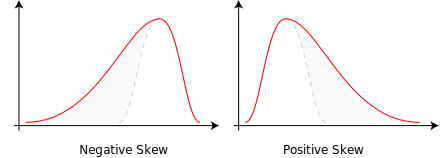
\includegraphics[width=0.8\linewidth]{img/Negative_and_positive_skew_diagrams_(English)}
	\caption{Same expectation and variance, but different skewness} 
\end{figure}
\end{frame}

\end{document}